\chapter{Analysis}
\label{ch:analysis}

This chapter is a comprehensive review of the tools, frameworks, and standards available to us. By conducting this analysis, we can identify the project constraints, evaluate the feasibility,
and decide on the project's design and implementation. Our project focuses on building a decentralized platform for international
settlements to provide a more efficient and cost-effective alternative to the current global settlement systems. As part of this analysis,
we aim to digitally create our own cryptocurrency token representing value within our platform. Additionally, our platform must be
able to facilitate the exchange of our cryptocurrency token for other cryptocurrencies and fiat currencies.

In section \ref{sec:ch2_ethereum}, we explore Ethereum as a decentralized application platform. We examine the Ethereum blockchain, its core features,
architecture, and the Ethereum Virtual Machine (EVM) role, enabling the execution of smart contracts. This section is fundamental to our project
as we will be using Ethereum as the foundation of our platform.

In section \ref{sec:ch2_solidity}, we delve into Solidity, the primary programming language used to develop smart contracts on the Ethereum blockchain.
We present its syntax, features, and how it facilitates the development of smart contracts of secure and robust smart contracts that will be used as the backend
of our platform.

In section \ref{sec:ch2_ethereum_token_standards}, we highlight the importance of token standards in the Ethereum ecosystem. We explore various token standards,
such as ERC-20, ERC-223, ERC-721, and ERC-777, and how they are used to create tokens on the Ethereum blockchain, and evaluate which token standard is best
suited for our platform cryptocurrency token.

In section \ref{sec:ch2_erc20}, we explore the ERC-20 token standard, the most widely used token standard in the Ethereum ecosystem. We analyze its features,
methods and how it aligns with our project requirements for creating versatile and interoperable tokens for international settlements and token exchange.

In section \ref{sec:ch2_openzeppelin}, we introduce OpenZeppelin, a reputable open-source framework for building secure smart contracts on the Ethereum blockchain.
We discuss how it can enhance the security and reliability of our smart contracts implementation, providing us with a solid foundation for building our
cryptocurrency token and ensuring a secure exchange of our token for other cryptocurrencies and fiat currencies.

The section \ref{sec:ch2_truffle} explores Truffle, a development environment and testing framework for Ethereum. We discuss the advantages of Truffle
for our project, including its ability to automate our smart contracts' compilation, deployment, and testing. It will aid us in efficiently developing
and deploying our decentralized platform.

Finally, section \ref{sec:ch2_web3} introduces Web3.js, a JavaScript library allowing our web application to interact with the Ethereum network.
We explain why web3.js is essential for our project, as it simplifies integrating Ethereum functionality into our frontend web application.
This allows us to interact with our cryptocurrency token and the Ethereum network.

% ----------------------------------------------------------------------------- DONE DONE

\section{Ethereum, a Decentralized Application Platform}
\label{sec:ch2_ethereum}

The Ethereum blockchain is a decentralized platform allowing us to develop and deploy decentralized applications (DApps) using smart contracts, which is 
revolutionary from Bitcoin's blockchain. Smart contracts, as their name suggests, are executed automatically under certain conditions,
preventing fraud or third-party interference. As described in the Ethereum white paper by Vitalik Buterin \cite{ethereum_white_paper}:

\begin{quote}
    \textit{The intent of Ethereum is to create an alternative protocol for building decentralized applications, providing a different set of tradeoffs that we
        believe will be very useful for a large class of decentralized applications, with particular emphasis on situations where rapid development time,
        security for small and rarely used applications, and the ability of different applications to very efficiently interact, are important.}
    
    \textit{(Vitalik Buterin, Ethereum White Paper, 2014)}
\end{quote}


Ethereum, compared to other blockchains, such as Bitcoin, is a more general-purpose blockchain. For example, while Bitcoin is a blockchain to transfer
value, Ethereum runs smart contracts. In addition, Ethereum is Turing-complete, which means that Ethereum is programmable.


% ----------------------------------------------------------------------------- DONE DONE


\subsection{Ethereum Accounts}

In Ethereum, there are two types of accounts, (1) \textit{externally owned accounts} and (2) \textit{contract accounts}. People can control externally owned accounts with their 
private keys protected with cryptography. On the other hand, contract accounts are held by their contract code. Therefore, they can only be activated by
an externally owned account, meaning that a contract account is one with which no private key is associated.
An account can transfer Ether to another account by creating a transaction, a message sent from one account to another.
In the Ethereum white paper \cite{ethereum_white_paper}, Vitalik Buterin describes an account as follows:

\begin{quote}
    \textit{...with each account having a 20-byte address and state transitions being direct transfers of value and information between
        accounts.}


    \textit{(Vitalik Buterin, Ethereum White Paper, 2014)}
\end{quote}

An Ethereum account contains four fields:

\begin{list}{-}{}
   \item \textbf{Nonce}: A counter used to make sure each transaction can only be processed once.
   \item  \textbf{Ether balance}: The number of Wei\footnote{1 Wei is the smallest denomination of Ether.} owned by the account.
   \item \textbf{Contract code}: The code is executed when the account receives a message call. It is mainly used for smart contracts.
   \item \textbf{Storage}: The storage of the account.
\end{list}


% ----------------------------------------------------------------------------- DONE DONE

\subsection{Messages and Transactions}
\label{subsec:messages_and_transactions}

For communicating between nodes, Ethereum uses two type of data structures, (1) \textit{messages} and (2) \textit{transactions}. A message is data that is sent from one contract
account to another contract account. A transaction is a signed data package sent from an externally owned account, which contains six fields: (1) the recipient of the transaction, (2) the signature of the transaction, (3) the amount of Ether to transfer,
(4) an optional data field, (5) a \texttt{STARTGAS} value, and (6) a \texttt{GASPRICE} value. The \texttt{GASPRICE} value represent a maximum amount of computational steps the transaction execution is allowed to execute.
The \texttt{GASPRICE} value is the fee the transaction's sender 
is willing to pay for each computational step. We explains with more details in the next section \ref{subsec:gas} and in section \ref{subsec:fees}, 
the \texttt{STARTGAS} and \texttt{GASPRICE} fields. 

Bitcoin and Ethereum have a similar transaction structure, because they both have the first three fields in common. The optional data field has no function in Ethereum. The \texttt{STARTGAS} and \texttt{GASPRICE} fields are
essential for preventing denial of service attacks. These fields are part of the anti-denial of the service model of Ethereum. The main goal of
the anti-denial of service model is to avoid situations where code execution is infinite or takes an extremely long time, accidentally
or intentionally.

With this gas and fees system, Ethereum assures that any attacker must pay for every resource he consumes. This mechanism is the core of the Ethereum,
allowing Ethereum to maintain the stability of its network and prevent malicious actors from spamming it.

% ----------------------------------------------------------------------------- DONE DONE

\subsection{Messages}

A message is described in the Ethereum white paper \cite{ethereum_white_paper} as follows:


\begin{quote}
   \textit{Messages are virtual objects that are never serialized and exist only in the Ethereum execution environment.}

   \textit{(Vitalik Buterin, Ethereum White Paper, 2014)}
\end{quote}


A message contains :


\begin{list}{-}{}
   \item \textbf{sender}: Sender of the message.
   \item \textbf{recipient}: Recipient of the message.
   \item \textbf{amount}: Amount of Ether to transfer.
   \item \textbf{data}: Optional data field.
   \item \textbf{STARTGAS}: Maximum number of computational steps the code execution is allowed to execute.
\end{list}


A message can be described as a transaction, but without the signature and the \texttt{GASPRICE} field, and is sent from one contract account to another
. Transactions and messages are processed similarly, but they have some differences. The main difference
is that a transaction is sent from an externally owned account, and a message is sent from a contract account. The other difference is that a transaction
can call a function that, as a result, creates a message and call another function in the same or another contract using the opcode \texttt{CALL} and \texttt{DELEGATECALL}
(see section \ref{sec:evm}). An amount of gas is used for a message sent from a transaction that triggers a function call.

% ----------------------------------------------------------------------------- DONE DONE

\subsection{Code Execution}
\label{sec:evm}

Smart contracts are described as a piece of code stored in the Ethereum blockchain world. To execute this code, we use a virtual machine called the Ethereum Virtual 
machine (EVM) that works as a Turing-complete virtual machine. The EVM can only understand bytecode. Therefore, we need to translate our code bytecode.
In the Ethereum white paper \cite{ethereum_white_paper}, Vitalik Buterin describes the code as follows:

\begin{quote}
   \textit{The code in Ethereum contracts is written in a low-level, stack-based bytecode language, referred to as "Ethereum virtual machine code" or "EVM code". The code consists of a series of bytes, each representing an operation.}

   \textit{(Vitalik Buterin, Ethereum White Paper, 2014)}
\end{quote}


In code execution, there is typically an infinite loop that follows a sequence of operations. The loop continuously operates as indicated
by the current program counter, which starts at zero. At the end of the execution of a function, the program counter is increased by one, and the next
operation is executed. Then, the process continues until one of the following conditions is met, (1) at the end of the code is reached, (2) when an error occurs or
(3) at the \texttt{STOP} or at \texttt{RETURN} instruction execution. The \texttt{STOP} instruction halts the execution of the code, and the \texttt{RETURN} instruction
returns the output data of the code execution. During execution, the EVM has access to three types of memory as illustrated in Figure \ref{fig:evm}:

\begin{figure}[H]
    \centering
    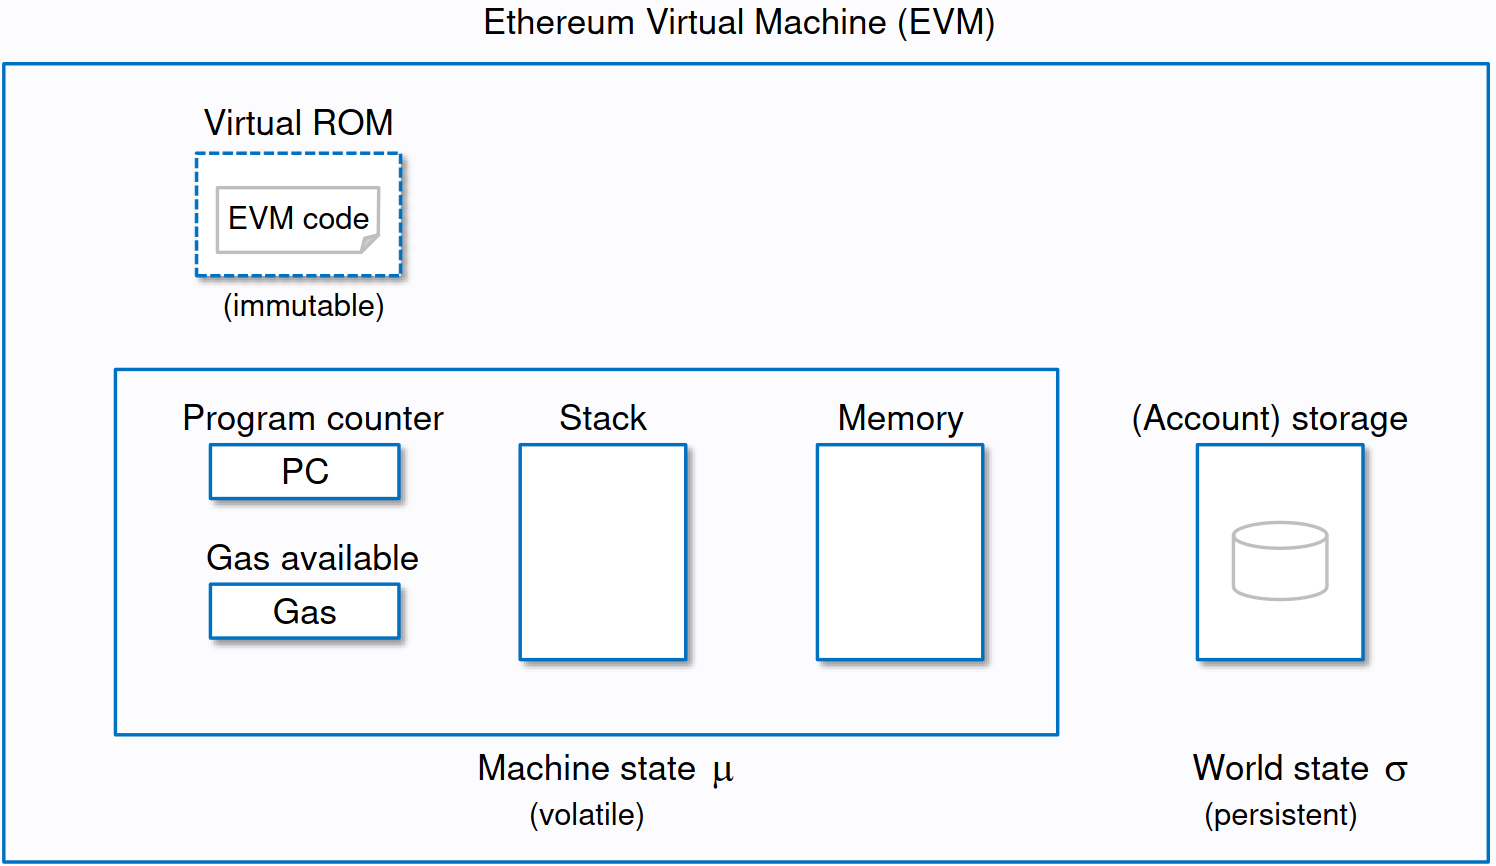
\includegraphics[width=1\columnwidth]{ch2/evm.png}
    \captionsource{Diagram of EVM architecture}
    {Diagram of EVM architecture as described in Ethereum Yellow Paper \cite{ethereum_yellow_paper}.
    }{\url{https://takenobu-hs.github.io/downloads/ethereum_evm_illustrated.pdf}}
    \label{fig:evm}
 \end{figure}

 Here is a description of the three types of memory illustrated in Figure \ref{fig:evm}:

\begin{list}{-}{}
   \item \textbf{Stack}: The stack is a last-in-first-out (LIFO) data structure and has a depth of 1024 items. It is used to store local variables.
   \item \textbf{Memory}: A byte array with a maximum size can represent the gas as a fuel of these of $2^{256} - 1$ bytes. The memory is used to store data.
   \item \textbf{Storage}: A key-value store with a maximum size of $2^{256} - 1$ key-value pairs. The storage is used to store data permanently even after the end
         of the computation, unlike the stack and the memory.
\end{list}


In addition, the code execution has access to the value, the sender, and the data of the message that triggered the code execution, as well as
the block header data. The code can return a byte array as output data. The output data is stored in the transaction that triggered the code execution.


% ----------------------------------------------------------------------------- DONE DONE

\subsection{Currency}
\label{subsec:currency_and_issuance}


The Ethereum white paper \cite{ethereum_white_paper} describes the currency and issuance as follows:

\begin{quote}
  \textit{The Ethereum network includes its own built-in currency, ether, which serves the dual purpose of providing a primary
      liquidity layer to allow for efficient exchange between various types of digital assets and, more importantly, of providing a
      mechanism for paying transaction fees.}

  \textit{(Vitalik Buterin, Ethereum White Paper, 2014)}
\end{quote}

The currency of Ethereum is called \textit{ether} and is used to pay for transaction fees and computational services. The smallest unit
of ether is called \textit{wei}. The denomination of ether is as follows:

\begin{table}[H]
  \centering
  \begin{tabular}{|l|l|l|}
      \hline
      % merge 3 cells in the first line
      \multicolumn{3}{|c|}{\textbf{Denonimation of Ether}}                 \\ \hline
      \textbf{Unit name} & \textbf{Value of Wei} & \textbf{Value of Ether} \\ \hline
      Wei (wei)          & $1$                   & $1\times10^{-18}$       \\ \hline
      $K$wei (babbage)   & $10^{3}$              & $1\times10^{-15}$       \\ \hline
      $M$wei (lovelace)  & $10^{6}$              & $1\times10^{-12}$       \\ \hline
      $G$wei (shannon)   & $10^{9}$              & $1\times10^{-5}$        \\ \hline
      $T$wei (szabo)     & $10^{12}$             & $1\times10^{-5}$        \\ \hline
      $P$wei (finney)    & $10^{15}$             & $1\times10^{-3}$        \\ \hline
      ether (buterin)    & $10^{18}$             & $1$                     \\ \hline
  \end{tabular}
  \caption{Ether denominations.}
  \label{tab:ether_denominations}
\end{table}


The wei denomination is designed for an internal representation of the data. The wei unit is used in most cases, and the values
are displayed in either denomination or other denominations in the user interface. It means the user does not need to
know the wei denomination to use the Ethereum network. Therefore, users interact with the Ethereum network using the ether denomination.


The Ethereum network has a fixed supply of ether, and the issuance of ether
is the way to create new ether. This process goes through mining\footnote{Mining is the process of adding new blocks to the blockchain.},
which involves solving a computationally difficult puzzle by miners\footnote{Miners are the nodes that participate in the mining process. They are
called miners because of the analogy with traditional mining, where miners are rewarded with gold for their work.}.
Miners contribute their computational power to the network and are rewarded with ether by successfully mining a block by solving the puzzle.
Note that the issuance of ether through mining has several purposes. First, it incentivizes miners to secure the network by validating transactions
and maintaining the integrity of the blockchain. Second, it ensures an adequate supply of ether, allowing actors to perform transactions and interact
with decentralized applications on the Ethereum network.




One core of the principles of Ethereum is the concept of \textit{Proof of Work} (PoW) consensus mechanism, where a fixed amount of ether is locked
for each successful block mined. Nevertheless, Ethereum plans to switch to a \textit{Proof of Stake} (PoS) consensus mechanism, known as
Ethereum 2.0. With the PoS consensus mechanism, the issuance of ether will occur through staking, where actors lock their ether as collateral to
participate in the consensus mechanism and receive rewards for their work. The Ethereum Foundation \cite{eth_proofofstake} explains the switch
to PoS as follows:


\begin{quote}
   \textit{The Ethereum network began by using a consensus mechanism that involved Proof-of-work (PoW). This allowed the nodes of the Ethereum network to agree on the state of all information recorded on the Ethereum blockchain
   and prevented certain kinds of economic attacks. However, Ethereum switched off proof-of-work in 2022 and started using proof-of-stake instead.}


   \textit{(Ethereum Foundation)}
\end{quote}


The issuance of new ether plays a crucial role in the functioning of the Ethereum network, providing necessary incentives for miners and ensuring
availability of ether for various transactions and interactions on the platform.



% ----------------------------------------------------------------------------- DONE DONE

\subsection{Gas}
\label{subsec:gas}


Gas is essential to the Ethereum network. The Ethereum white paper \cite{ethereum_white_paper} describes gas as follows:


\begin{quote}
   \textit{In order to prevent accidental or hostile infinite loops or other computational wastage in code, each transaction is
       required to set a limit to how many computational steps of code execution it can use. The fundamental unit of computation is "gas";
       usually, a computational step costs 1 gas, but some operations cost higher amounts of gas because they are more computationally expensive,
       or increase the amount of data that must be stored as part of the state.}


   \textit{(Vitalik Buterin, Ethereum White Paper, 2014)}
\end{quote}

We can represent the gas as a fuel of the Ethereum network, measuring the amount of work required to perform a specific operation.
Each transaction requires a certain amount of resources to be executed. Thus each transaction requires a \textit{fee}  to
execute a transaction or a message in Ethereum even if the transaction succeeds or fails.

\begin{figure}[H]
   \centering
   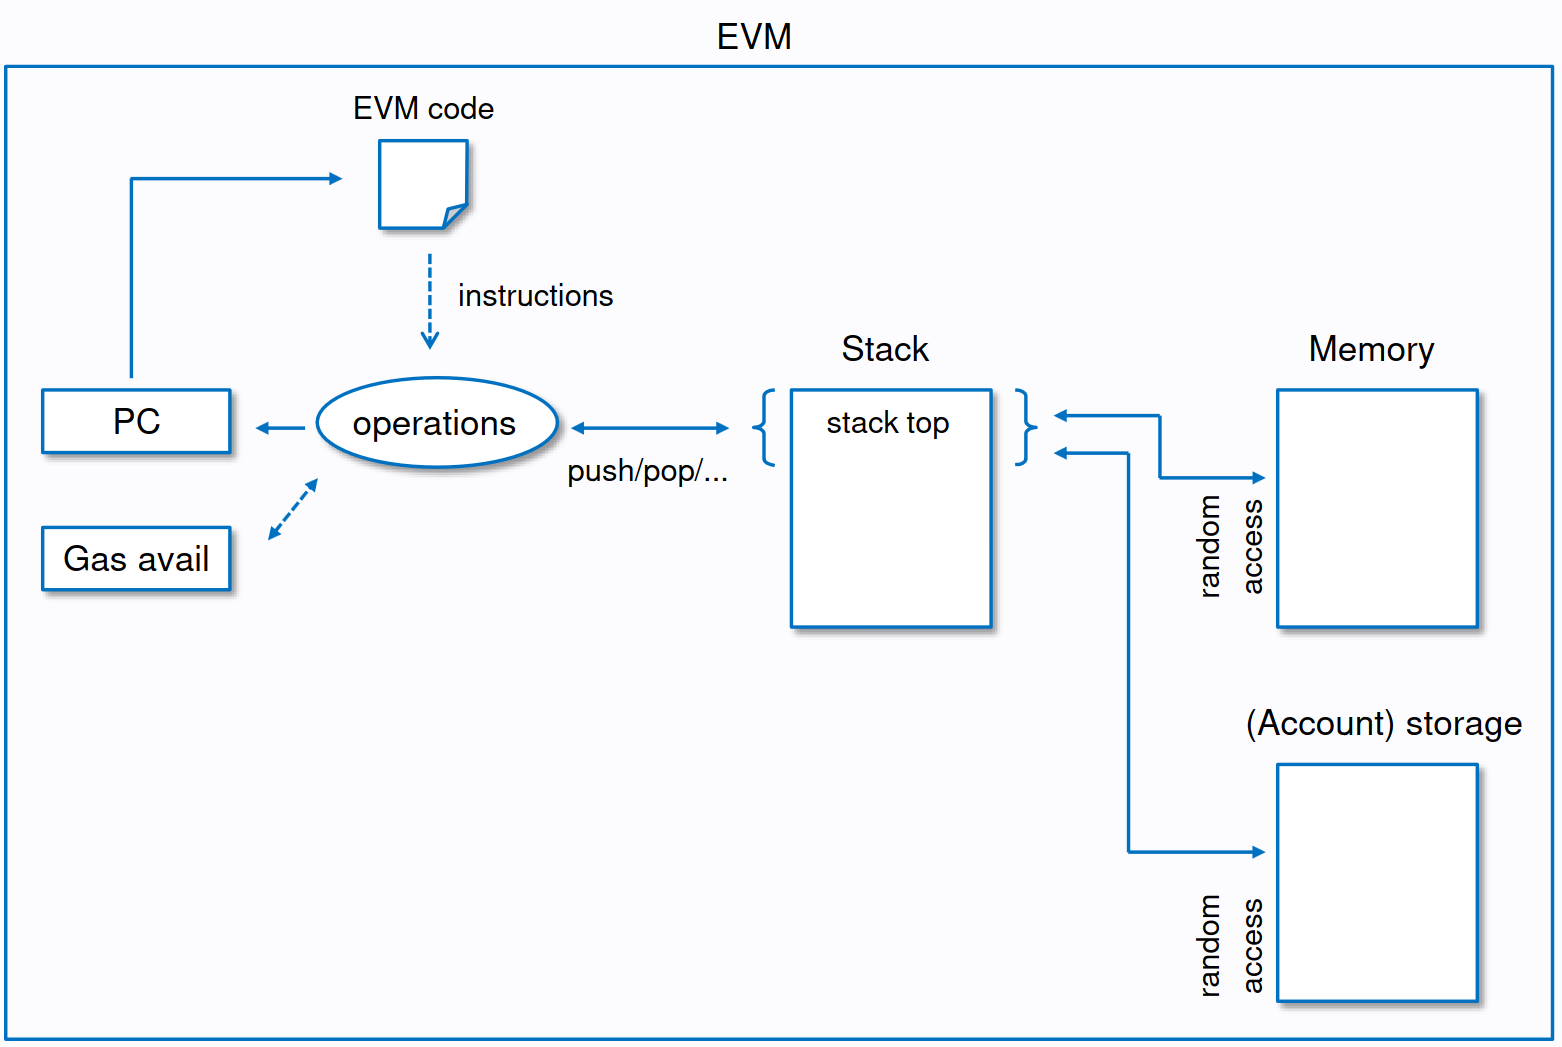
\includegraphics[width=0.8\textwidth]{ch2/gas.png}
   \captionsource{Diagram of execution model }
   {Diagram of execution model as described in Ethereum Yellow Paper \cite{ethereum_yellow_paper}.}
   {\url{https://takenobu-hs.github.io/downloads/ethereum_evm_illustrated.pdf}}
   \label{fig:gas}
\end{figure}


Figure \ref{fig:gas} above shows the execution model of the Ethereum Virtual Machine, where the gas is used to pay for the execution of the code. Another
value is \texttt{GASLIMIT}. This value is the maximum amount of gas used on a transaction. For example, some complicated transactions may require more gas than the
default gas limit. If the gas limit is too low, the transaction will fail, and the gas will be consumed. Standard transactions have a gas limit of 21,000 gas.


% ----------------------------------------------------------------------------- DONE DONE

\subsection{Fees}
\label{subsec:fees}


As in Bitcoin, the fees are a crucial part of the Ethereum network because they prevent the network from being overloaded by computations. The difference between Bitcoin 
and Ethereum is that in Bitcoin, the fees are paid per byte of data, whereas in Ethereum, the fees are paid per computational step. As mentioned in the previous section 
\ref{subsec:gas}, the gas is used to prevent infinite loops or other computational wastage in code.The \texttt{STARTGAS} (see section \ref{subsec:messages_and_transactions}) 
value represents the maximum amount of gas, meaning we cannot exceed a certain number of computational steps. Every transaction requires a limit of gas to prevent infinite loops, and each computational step costs a certain 
amount of gas, typically one gas. However, some operations cost more due to their computational complexity or due to storage space.

The fee is integral to each transaction and serves as a deterrent against spam attacks. Transactions requiring more resources will incur higher fees than those with fewer resources, making the fee proportional to the transaction size. The calculation of the transaction fee is demonstrated by the equation below.


\begin{equation}
   \label{eq:transaction_fee}
   \text{Transaction Fee} = \texttt{STARTGAS} \times \texttt{GASPRICE}
\end{equation}


One advantage of decoupling the execution cost from a specific currency, such as setting the cost of a computation step to three wei, is separating transaction 
execution cost from the fluctuations in Ether's value compared to fiat currencies. For example, if the price of Ether significantly rises relative to a currency like a 
dollar, a fixed price per computational step could become unaffordable. To address this concern, the \texttt{GASPRICE} (see section \ref{subsec:messages_and_transactions}) 
is used to set the gas price in Ether, ensuring a consistent amount of gas consumed by the transaction while allowing for adjustments in the overall gas price.

% ----------------------------------------------------------------------------- DONE DONE


\section{Solidity, a high-level language for Ethereum}
\label{sec:ch2_solidity}


To interact with the Ethereum network, we need to write smart contracts. For this purpose, we use Solidity, a high-level language for
implementing smart contracts. Solidity is a statically typed language that supports inheritance, libraries, and complex user-defined types, among other features.
From the official documentation \cite{ethereum_solidity_doc}, Ethereum foundation describes Solidity as follows:


\begin{quote}
   \textit{Solidity is an object-oriented, high-level language for implementing smart contracts. Smart contracts are programs that govern the behavior of accounts within the Ethereum state.
       Solidity is a curly-bracket language that targets the Ethereum Virtual Machine (EVM). C++, Python, and JavaScript influence it. In the language influences section, you can find more details about which languages Solidity has been inspired by.}


   \textit{(Ethereum Foundation)}
\end{quote}


Solidity owns its compiler, the compiler \textit{solc}, whose purpose is to translate the Solidity code into bytecode, the only language understood by the Ethereum Virtual Machine (EVM). 
Developed in C++, the Solidity compiler is licensed under the GNU Lesser General Public License v3.0 (LGPL). It offers both command-line utility and library 
functionalities, providing flexibility in its usage.

In summary, all smart contracts for our project are written in Solidity and compiled into EVM-executable bytecode. The upcoming sections will delve into the Solidity 
language and discuss the fundamental structure necessary to understand how we implemented smart contracts in our project.

% ----------------------------------------------------------------------------- DONE DONE

\subsection{State Variables}

State variables in Solidity are a contract's persistent data stored on the blockchain, retaining their values throughout multiple function calls. These 
variables define the properties and attributes of a contract and are accessible to all functions within it.

To declare a state variable in Solidity, we specify its type, visibility, and optional modifiers. Solidity offers a range of data types, including integers, booleans, 
strings, arrays, structs, and user-defined types. These data types enable the representation and manipulation of different kinds of data within the smart contract.

\begin{listing}[H]
    \begin{minted}[]{solidity}
// SPDX-License-Identifier: GPL-3.0
pragma solidity ^0.8.0;

contract SimpleStorage {
    uint256 public storedData;
    string public name = "SimpleStorage";

    function set(uint256 x) public {
        storedData = x;
    }

    function get() public view returns (uint256) {
        return storedData;
    }
}
    \end{minted}
    \caption{Example of a contract with a state variable.}
    \label{lst:state_variable}
\end{listing}

In the Listing \ref{lst:state_variable}, the contract \texttt{SimpleStorage} has a state variable \texttt{storedData} of type \texttt{uint256}.
By utilizing state variables, Solidity provides a powerful mechanism for managing and preserving the state of blockchain contracts, facilitating decentralized applications' development.

% ----------------------------------------------------------------------------- DONE DONE

\subsection{Functions}

Functions in Solidity play a crucial role in implementing the logic of a contract and are similar to functions in other programming languages. They can 
be declared with different visibilities, including \texttt{external}, \texttt{public}, \texttt{internal}, or \texttt{private}. The default visibility is \texttt{public}.


\begin{listing}[!ht]
    \begin{minted}[]{solidity}
// SPDX-License-Identifier: GPL-3.0
pragma solidity ^0.8.0;

contract MySimpleFunction {
    constructor() {
        // constructor
    }

    function mint(address account, uint256 amount) public onlyOwner {
        _mint(account, amount);
    }

    function decimals() public view virtual override returns (uint8) {
        return 2;
    }

}
    \end{minted}
    \caption{Example of a contract with a function.}
    \label{lst:function}
\end{listing}

In the provided Listing \ref{lst:function}, we show a contract named \texttt{MySimpleFunction} that implements two functions: \texttt{mint} and \texttt{decimals}.
The \texttt{mint} function is declared as \texttt{public}, allowing anyone to call it. It is responsible for minting tokens by invoking the \texttt{\_mint} function.
On the other hand, the \texttt{decimals} function is declared as \texttt{public view}, indicating that anyone can call it and only reads data from the contract without
modifying the state. In this case, the \texttt{decimals} function returns the number of decimals for the token without requiring a transaction and, therefore, is free of
charge of gas.

% ----------------------------------------------------------------------------- DONE DONE

\subsection{Function Modifiers}

\begin{listing}[!ht]
    \begin{minted}[]{solidity}
// SPDX-License-Identifier: GPL-3.0
pragma solidity ^0.8.0;

contract MyToken{
    address public owner;
    
    modifier onlyOwner() {
        require(msg.sender == owner, "Only owner can call this function.");
        _;
    }

    constructor() {
        owner = msg.sender;
    }

    function transferOwnership(address newOwner) public onlyOwner {
        owner = newOwner;
    }
}
    \end{minted}
    \caption{Example of a contract with a function modifier.}
    \label{lst:modifier}
\end{listing}


In the Listing \ref{lst:modifier}, the contract \texttt{MyToken} has a function modifier \texttt{onlyOwner}. The function modifier \texttt{onlyOwner} restricts
access to certain functions. In this case, only the owner of the contract can call the function \texttt{transferOwnership}.
The variable \texttt{msg.sender} is a global variable that contains the address of the sender of the message. The underscore (\texttt{\_}) in the function modifier
indicates where the function body will be executed.


% ----------------------------------------------------------------------------- DONE

\subsection{Events}

Events are used to notify external applications about the occurrence of a specific event. This allows direct interaction with EVM logs.
Events are an essential part of the Ethereum ecosystem because they allow to interact with smart contracts in a decentralized way, for example
dApps (Decentralized Applications) and Oracles\footnote{Oracles are third-party services that provide smart contracts with external information.}.

\begin{listing}[!ht]
   \begin{minted}[]{solidity}
// SPDX-License-Identifier: GPL-3.0
pragma solidity ^0.8.0;


contract MyTokenAction{
   event Transfer(address indexed from, address indexed to, uint256 value);


   function transfer(address _to, uint256 _value) public returns (bool success) {
       emit Transfer(msg.sender, _to, _value);
       return true;
   }
}
   \end{minted}
   \caption{Example of a contract with an event.}
   \label{lst:event}
\end{listing}


In Listing \ref{lst:event}, the contract \texttt{MyTokenAction} shows the usage of an event called \texttt{Transfer}. The \texttt{Transfer} event serves to notify external applications about the transfer of tokens. The \texttt{transfer} function, responsible for transferring tokens from one address to another, emits the
\texttt{Transfer} event after completing the token transfer. The \texttt{emit} keyword triggers the event, providing the necessary arguments.

% ----------------------------------------------------------------------------- DONE DONE

\subsection{Structs}

Structs in Solidity serve as a mechanism for defining custom data types. They are similar to structs in C or C++ and are utilized to group variables, creating a cohesive 
data structure. As a result, structs are particularly valuable for organizing and storing data within smart contracts.


\begin{listing}[!ht]
    \begin{minted}[]{solidity}
// SPDX-License-Identifier: GPL-3.0
pragma solidity ^0.8.0;

contract Orderbook {

    struct Order {
        uint amount;
        uint price;
        uint timestamp;
        address trader;
        bytes2 status;
    }
}
    \end{minted}
    \caption{Example of a contract with a struct.}
    \label{lst:struct}
\end{listing}

In Listing \ref{lst:struct}, we present the contract \texttt{Orderbook}, which incorporates a struct named \texttt{Order}. 
This struct is responsible for storing order-related data. Within the \texttt{Order} struct, several properties are defined, including \texttt{amount}, \texttt{price}, 
\texttt{timestamp}, \texttt{trader}, and \texttt{status}. By utilizing the \texttt{Order} struct, the contract can effectively store and manage order data within the 
order book.

% ----------------------------------------------------------------------------- DONE DONE

\subsection{Common Data Types in Solidity}

Solidity supports various data types that allow developers to define and manipulate variables within smart contracts. Here are some common data types used in Solidity:

\begin{itemize}
   \item \textbf{Integers}: Solidity provides signed and unsigned integer types with different bit sizes. We can specify the number of bits by appending the number, such as \texttt{uint256} or \texttt{int8}.


   \item \textbf{Booleans}: Solidity includes a \texttt{bool} type that can store either \texttt{true} or \texttt{false}.


   \item \textbf{Bytes}: Solidity provides a \texttt{bytes} type that can be used to store byte arrays. For example, \texttt{bytes32} represents a byte array of 32 bytes. The \texttt{bytes} type is similar to the \texttt{string} type, but it is not UTF-8 encoded and does not support string operations.


   \item \textbf{Address}: The \texttt{address} type represents a 20-byte Ethereum address. It can store Ethereum and contract addresses and provides various member functions to interact with.


   \item \textbf{Strings}: Solidity supports string types (\texttt{string}) for storing and manipulating variable-length text data.


   \item \textbf{Arrays}: Solidity allows the declaration of fixed-size and dynamic arrays. Fixed-size arrays have a predefined length, such as \texttt{uint[5]} for an array of five unsigned integers. Dynamic arrays can have a variable length, such as \texttt{uint[]} for an array of unsigned integers.


   \item \textbf{Mappings}: Solidity provides mappings and key-value stores that associate values with unique keys. Mappings can be used to implement data storage and retrieval efficiently. For example, \texttt{mapping(address => uint)} represents a mapping that associates unsigned integers with addresses.


   \item \textbf{Enums} allows us to define a set of named constants. Each constant has an associated integer value. Enums help define states or options within a contract.


   \item \textbf{Function Types}: Solidity supports function types, which enable us to declare variables or parameters that can store or refer to functions. Function types help implement callback mechanisms or pass functions as arguments.


\end{itemize}

These data types have been selected based on their relevance to our project and are commonly used to develop smart contracts. Using these data types in our project ensures efficient and secure data handling within the contract.
It is important to note that Solidity offers a broader range of data types beyond those mentioned in this list. The official Solidity documentation \cite{ethereum_solidity_doc} refers to a comprehensive understanding of all 
available data types and their specific use cases.

% ----------------------------------------------------------------------------- DONE DONE

\subsection{UML Diagram for Solidity Code}

Unified Modeling Language (UML) diagrams are graphical representations that visualize the structure and relationships of various elements
in software systems. While UML diagrams are commonly used for object-oriented programming languages, they can also be adapted to represent
Solidity code. This project uses UML diagrams to describe the structure and relationships between our Token and exchange contracts.
To create UML diagrams in \LaTeX, we use the \texttt{tikz-uml} package. This package provides a set of macros for creating UML sequence diagrams, class diagrams, 
and other UML diagram types.


Here is an example of how to represent a UML class diagram for Solidity code using the \texttt{tikz-uml} package:


\begin{figure}[H]
   \centering
   \begin{tikzpicture}[scale=0.8, transform shape]
       \begin{umlpackage}{MyToken}
           \umlclass{MyToken}{}{
               + owner: address \\
               \umlstatic{-- onlyOwner() : modifier} \\
               \umlstatic{+ transferOwnership(newOwner: address) : void}
           }


           \umlclass[x=3,y=-5]{address}{}{}


           \umlaggreg[mult1=1,pos1=0.2,mult2=1,pos2=0.8]{MyToken}{address}
           \umluniassoc[arg1=owner,arg2=address,pos=0.5]{MyToken}{address}


           \umlnote[x=0,y=-7,width=7.5cm]{MyToken}{\textbf{Note:} The \texttt{onlyOwner()} function is a modifier in the \texttt{MyToken} contract that ensures the owner of the contract can only execute some functions.}
       \end{umlpackage}
   \end{tikzpicture}
   \caption{UML Class Diagram for Solidity Code}
   \label{fig:uml_diagram}
\end{figure}

Figure \ref{fig:uml_diagram} shows a UML class diagram for the Solidity code presented in the Listing \ref{lst:function}. The \texttt{tikz-uml} package provides macros
for creating UML classes, sequences, and other UML diagram types.

\begin{figure}[H]
    \centering
    \begin{tikzpicture}[thick]
        \begin{umlseqdiag}
            % Participant: Owner
            \umlactor[class=Owner,,fill=white!0]{Alice}

            % Participant: Contract
            \umldatabase[class=Contract,fill=white!0,x=5]{MyToken}

            % Alice calls transferOwnership(Bob)
            \begin{umlcall}[op={transferOwnership(Bob)}, return=emit OwnershipTransferred, draw=SkyBlue, fill=SkyBlue!20, dt=5]{Alice}{MyToken}
                % Contract calls onlyOwner()
                \begin{umlcallself}[op={onlyOwner()}, fill=ForestGreen!20, draw=ForestGreen, return=true]{MyToken}
                \end{umlcallself}
            \end{umlcall}

            % Alice attempts to transfer ownership again, but it fails
            \begin{umlcall}[op={transferOwnership(Alice)},return=revert, draw=SkyBlue,fill=SkyBlue!20, dt=5]{Alice}{MyToken}
                % Contract calls onlyOwner()
                \begin{umlcallself}[op={onlyOwner()}, fill=ForestGreen!20, draw=ForestGreen, return=false]{MyToken}
                \end{umlcallself}
            \end{umlcall}

            % Transaction indicator
            \filldraw[draw=SkyBlue,fill=SkyBlue!20] (1.2,-5) circle (.2);
            \node at (0,-5) {Transaction};

            % Call indicator
            \filldraw[draw=ForestGreen,fill=ForestGreen!20] (3,-5) circle (.2);
            \node at (3.6,-5) {Call};
        \end{umlseqdiag}
    \end{tikzpicture}
    \caption{UML Sequence Diagram for presenting the function \texttt{transferOwnership}.}
    \label{fig:uml_sequence_diagram}
\end{figure}


Figure \ref{fig:uml_sequence_diagram} illustrates a UML sequence diagram corresponding to the Solidity code presented in Listing \ref{lst:function}. The diagram captures 
the sequence of interactions between the actors, Alice and Bob, and the contract's functions.
In the diagram, Alice initiates the process by calling the function \texttt{transferOwnership}, which transfers her ownership to Bob. This function internally invokes the 
\texttt{onlyOwner} modifier to verify whether the caller is the contract owner. If the caller is not the owner, the \texttt{onlyOwner} function reverts the transaction, 
preventing the transfer of ownership. The transaction is reverted in this scenario because Alice is not the contract owner since she has already transferred her right to Bob.
The diagram distinguishes between transactions and calls using different colors. For example, blue circles represent transactions, while calls are depicted with green circles.
This UML sequence diagram provides a visual representation of the interactions and control flow within the contract, aiding in understanding its functionality and behavior.

% ----------------------------------------------------------------------------- DONE DONE

\section{Ethereum Token Standards}
\label{sec:ch2_ethereum_token_standards}

In blockchain technology and cryptocurrencies, a token is essential in allowing more possibilities and use cases of decentralized
applications and ecosystems. A token represents a digital asset that can be compared in various forms of value, such as money, gold, certificates, and more.
To enable interoperability, consistency, and compatibility between different tokens, the Ethereum community has created a set of token standards.
These standards are called Ethereum Request for Comments (ERC). The ERC standards are Ethereum Improvement Proposals (EIP) that define a set of rules
that a token must implement to be ERC-compliant.


This section focuses on presenting token standards with a particular focus on the Ethereum blockchain. The Ethereum platform is
known for its innovative contract capabilities and therefore is a pioneer in creating token standards through EIPs.
Their proposals define the specifications and norms that a token must follow, ensuring uniformity and facilitating the integration
of tokens in different applications.


In the following subsections, we describe the concept of a token, providing a general overview of the token standards. Then, we present
the Ethereum Improvement Proposals created to define the token standards. Finally, we explore some of the cryptocurrency ecosystem's most popular
token.


% ----------------------------------------------------------------------------- DONE DONE

\subsection{What is a Token ?}

A token digitally represents an asset or utility within a decentralized network. It is often created and issued by
a smart contract, a self-executing contract of rules with predefined conditions on the blockchain. We can compare a token
to a physical token in the real world, where a token can represent ownership rights or access to a service. In the Ethereum Whitepaper
\cite{ethereum_white_paper}, Vitalik Buterin defines a token as follows:

\begin{quote}
   \textit{On-blockchain token systems have many applications ranging from sub-currencies representing assets such as USD or gold to
       company stocks, individual tokens representing smart property, secure unforgeable coupons, and even token systems with no ties to
       conventional value at all, used as point systems for incentivization.}


   \textit{(Vitalik Buterin, Ethereum Whitepaper)}
\end{quote}


We can illustrate the concept of a token with an example. First, let us consider an analogy for an IT Security convention like the DEF CON
\footnote{DEFCON is one of the world's largest hacker conventions, held annually in Las Vegas, Nevada.} convention. Imagine we attend
the DEFCON convention, and as we enter the convention, we receive a special badge that gives us certain privileges. This badge
is similar to a token because it allows us to access certain convention areas, participate in exclusive events, and receive certain benefits. However, in this case, the badge represents a value within the DEFCON convention, enabling us to engage
in certain activities.

We can cite some examples of tokens such as Aragon (ANT)\footnote{Aragon Token: \url{https://aragon.org/}} and Basic Attention Token (BAT)\footnote{Basic Attention Token: \url{https://basicattentiontoken.org/}}.
Aragon provides governance rights within the Aragon Network. Holding Aragon tokens gives the holder the right to vote on certain
decision-making processes and influence the direction of the project.

From a business perspective, a token can offer the company a new opportunity to issue shares, securities, or their own
currency, allowing them to take control of their finances. In addition, companies can use tokens to get exclusive access to certain services
or products within their ecosystem. For example, many companies use tokens to raise project funds through Initial Coin Offerings (ICO)\footnote{ICO: \url{https://en.wikipedia.org/wiki/Initial_coin_offering}}.
An ICO is a fundraising mechanism in which new projects sell their underlying crypto tokens in exchange for bitcoin and ether. It is
similar to an Initial Public Offering (IPO)\footnote{IPO: \url{https://en.wikipedia.org/wiki/Initial_public_offering}},
 in which investors purchase company shares. Creating a cryptocurrency token for
international settlements allows companies to avoid intermediaries and reduce costs and transaction time. However, regulatory compliance is
critical for companies that want to issue tokens with specific characteristics.


% ----------------------------------------------------------------------------- DONE DONE

\subsection{Ethereum Improvement Proposals}
\label{subsec:eip}

The Ethereum Improvement Proposals (EIP) are crucial in defining standards and guidelines for token creation and implementation on the Ethereum
platform. EIPs are formal documents submitted by Ethereum community members (like developers and researchers) to propose improvements
, new features, and changes to the Ethereum protocol.


Regarding token standards, the Ethereum Requests for Comments (ERC) are EIPs that define a set of rules that a token must implement on the Ethereum
platform to adhere to the standard. It ensures that the tokens created are compatible and interoperable among different projects and applications.
ERCs are defined as a significant contribution to the Ethereum ecosystem and are widely used by the community. The official documentation
for ERCs can be found on the Ethereum GitHub repository\footnote{Ethereum GitHub repository: \url{https://github.com/ethereum/EIPs}}.
The ERC20 is by far the most popular token standard for fungible tokens\footnote{Fungible tokens are interchangeable and can be replaced by another token.},
offering consistency and integration for developers. In addition, ERC20 can represent any digital asset, such as cryptocurrencies, loyalty points, and gold certificates.


In addition to the ERC20, other token standards are widely used in the Ethereum ecosystem. We can cite notable token standards
such as the ERC721, introducing non-fungible tokens (NFTs)\footnote{Non-fungible tokens are unique and indivisible tokens that another token cannot replace.}
, which are unique and indivisible digital assets. NFTs are widespread in gaming, art, and collectibles, enabling
verifiable digital ownership and scarcity.


There are a lot of other token standards that are widely used in the Ethereum ecosystem. We can cite some examples, such as the ERC777 and ERC1155.
Ethereum Improvement Proposals and token standards have significantly contributed to the Ethereum ecosystem's growth and development, enabling
innovation, facilitating token creation, and diverse, decentralized applications on the Ethereum blockchain.


% ----------------------------------------------------------------------------- DONE DONE

\subsection{Token standards}

As explained in the previous section \ref{subsec:eip}, the most approved token standard is the ERC20 which we describe more in detail in the section \ref{sec:ch2_erc20}.
Many other token standards are designed from the ERC20 for (1) suggesting improvements, (2) adding new features, (3) solving problems, or (4) proposing new functionalities.
Some proposals define entirely new token standards, such as the ERC777. The table \ref{tab:token_standards} shows some of the most popular token standards derived from the ERC20.

\begin{table}[h]
   \rowcolors{1}{gray!15}{white} % Set row colors, starting from the first row
   \begin{tabular}{|c|p{5cm}|p{3cm}|p{2cm}|}
       \hline
       \rowcolor{gray!50} % Set header row color
       \textbf{Token Standard} & \textbf{Description}                                                                                                                          & \textbf{Author}                                    & \textbf{Date} \\
       \hline
       ERC-20                  & The standard for fungible tokens on the Ethereum blockchain, ensuring interoperability and ease of integration.                               & Fabian Vogelsteller and Vitalik Buterin            & November 2015 \\
       \hline
       ERC-223 (Draft)         & An improvement over ERC-20, introducing enhanced security features and efficiency, including the ability to reject incoming token transfers.  & Dexaran                                            & March 2017    \\
       \hline
       ERC-777                 & A more advanced token standard that fixes some of the issues with ERC-20, including the sending mechanism for regular accounts and contracts. & Jordi Baylina, Jacques Dafflon, and Thomas Shababi & November 2017 \\
       \hline
       ERC-827                 & An extension of ERC-20, providing additional functionalities like approving token transfers on behalf of the token holder.                    & Joseph Chow                                        & January 2018  \\
       \hline
   \end{tabular}
   \caption{List of some  EIPs token standards derived from the ERC20.}
   \label{tab:token_standards}
\end{table}

Table \ref{tab:token_standards} provides an overview of token standards, illustrating that the ERC20 token standard was the first to be established in November 2015.
Subsequently, other token standards have emerged, building upon the foundation set by ERC20. It is important to note that the table represents a selection and is not exhaustive. To explore the complete documentation and comprehensive lists of token standards, one can visit the official website of Ethereum Improvement Proposals (EIPs)
\cite{ethereum_eip}. The EIPs website is a valuable resource for the community, providing access to drafts and proposals open for review and discussion.

% ----------------------------------------------------------------------------- DONE DONE

\section{ERC20 Token Standard}
\label{sec:ch2_erc20}

This section introduces the importance of selecting appropriate token standards for our settlement solution. Tokens serve as a medium of exchange and can represent any digital asset
such as cryptocurrencies, enabling seamless and secure transactions. With numerous tokens at our disposal, the ERC20 token standard is the most popular and widely adopted choice for
fungible tokens because of its simplicity and interoperability. We provide an overview of the ERC20 token standard, explaining its functionalities and features.

% -----------------------------------------------------------------------------

\subsection{Overview of ERC20}

The ERC20 token standard stands for Ethereum Request for Comments 20 and has been proposed by Fabian Vogelsteller and Vitalik Buterin in 19\textsuperscript{th} November 2015 \cite{eth_erc20}.
It introduces a standardized interface for fungible tokens on the Ethereum blockchain, ensuring interoperability and ease of integration among different projects. ERC20 tokens are
designed to be interchangeable and can be replaced by any other token of the same type and exchanged on a one-to-one basis. This particular feature called fungibility makes ERC20
tokens suitable for representing currencies, digital assets, and other financial instruments where uniformity and interchangeability are vital. This allows developers to
create decentralized applications (DApps) that can interact with any ERC20 token without implementing custom code for each token. The ERC20 interface specifies a set of functions
called ERC20 methods that the token contract must implement. The methods allow actors to transfer their tokens to other addresses, get the current token balance of an address, and approve
the transfer of tokens from one address to another. The following code snippet shows the ERC20 interface in Solidity from the EIP-20 \cite{eth_erc20}.

\begin{listing}[!ht]
   \begin{minted}[]{solidity}
interface IERC20 {
   function name() external view returns (string memory);
   function symbol() external view returns (string memory);
   function decimals() external view returns (uint8);
   function totalSupply() external view returns (uint256);
   function balanceOf(address account) external view returns (uint256);
   function transfer(address recipient, uint256 amount) external returns (bool);
   function transferFrom(address sender, address recipient, uint256 amount) external returns (bool);
   function allowance(address owner, address spender) external view returns (uint256);
   function approve(address spender, uint256 amount) external returns (bool);
   event Transfer(address indexed from, address indexed to, uint256 value);
   event Approval(address indexed owner, address indexed spender, uint256 value);
}
   \end{minted}
   \caption{ERC20 interface presented in Solidity.}
   \label{lst:erc20_interface}
\end{listing}


The listing \ref{lst:erc20_interface} shows the ERC20 interface in Solidity representing nine functions and two events. The functions are described as follows:


\begin{itemize}
    \item \mintinline{solidity}|name()|: Returns the token's name as the name suggests. E.g. the name of \textit{Universal Export Token} is \texttt{Universal Export Token}.
    \item \mintinline{solidity}|symbol()|: Returns the token's symbol, usually a shorter name version. E.g. the symbol of \textit{Universal Export Token} is \texttt{UET}.
    \item \mintinline{solidity}|decimals()|: Returns the representation of the smallest fraction of a token because of the absence of floating-point numbers in Solidity. If \texttt{decimals} returns $2$, 
    a balance of 12345 tokens should be displayed to a user as $123.45$.
    \item \mintinline{solidity}|totalSupply()|: Returns the total token supply.
    \item \mintinline{solidity}|balanceOf(address)|: Returns the token balance of a given address.
    \item \mintinline{solidity}|transfer(address, amount)|: Transfers a specified amount of tokens from the sender's address to the recipient's address. The function returns a boolean
          value indicating whether the operation was successful and must fire the \mintinline{solidity}|Transfer| event. The return value of 0 indicates that the transfer was successful.
    \item \mintinline{solidity}|transferFrom(from, to, amount)|: Transfers a specified amount of tokens from one address to another. The function returns a boolean value
          indicating whether the operation was successful and must fire the \mintinline{solidity}|Transfer| event. This method is used for a withdrawal workflow,
          meaning a user can transfer tokens on behalf of another user (e.g., a decentralized exchange) with charge fees.
    \item \mintinline{solidity}|allowance(owner, spender)|: Returns the current allowance of a spender for a given owner. The allowance is the maximum amount of tokens a spender can spend on behalf of the owner.
    \item \mintinline{solidity}|approve(spender, amount)|: Allows a spender to transfer a specified amount of tokens on behalf of the token owner.
    \item \mintinline{solidity}|Transfer(address, address, amount)|: Emitted when tokens are transferred from one address to another. The event is triggered when tokens are transferred by the \mintinline{solidity}|transfer| and \mintinline{solidity}|transferFrom| functions.
    \item \mintinline{solidity}|Approval(address, address, amount)|: Emitted when the allowance of a spender for an owner is set by the \mintinline{solidity}|approve| function. The event is triggered when the allowance is set by the \mintinline{solidity}|approve| function.
\end{itemize}

All balances and amount parameters are represented on 256 bits of unsigned integers. Thus, the maximum amount of tokens that can be handled is $2^{256} - 1$. The point is to make that some functions are declared as \texttt{view} functions
like \mintinline{solidity}|name()|, \mintinline{solidity}|symbol()|, etc. It indicates that the function does not modify the state of the contract and does not consume any gas. Therefore the \texttt{view} functions are free to call and do not require gas.
It can be compared to a getter function in object-oriented programming that returns a private variable's value. Another critical point is the \mintinline{solidity}|decimal()| function. When working
with tokens, we usually work with a small amount, representing a fraction of a token. For example, if one owns 4 UET tokens, transferring 3.49 UET to another address may be necessary, and keeping 0.51 UET in the sender's address. The EVM does not support floating point numbers, so Solidity allows us to define the integer number values of the token that should be displayed as a fraction of a token.
It can be a problem because if one wants to transfer 3.49 UET, the number of tokens to transfer can be only 3 UET or 4 UET.

To solve this problem, ERC20 tokens include the \mintinline{solidity}|decimals()| function that returns the representation of the smallest fraction of a token with
an integer value. For example, if \mintinline{solidity}|decimals()| equals $2$, it can transfer 3.49 UET by transferring 349 UET and keeping 51 UET in the sender's address. It is important to note that the \mintinline{solidity}|decimals()| function is only used for display purposes
and does not affect the arithmetic of the token. A decimal value of 2 is usually common in many other ERC20 tokens. It means when we mint or transfer tokens, we work with a value of :

\begin{center}
    \begin{equation}
        \centering
        \text{value} = \text{UET} \times 10^{\text{decimals}}
    \end{equation}
    \label{eq:decimals}
 \end{center}
 
 
 For example, if we want to mint 1000 UET, we mint $1000 \times 10^2 = 100000$ UET, the same process for transferring tokens. However, some tokens
 like Ether have a decimal value of 18, which means that when we transfer 1 Ether, we transfer $1 \times 10^{18} = 1000000000000000000$ Wei. Some others have a decimal value of 0,
 which means that when we transfer 1 token, we transfer $1 \times 10^0 = 1$ token. It can make sense for some tokens like a token representing a share of a company. However, it is not possible to transfer
 a fraction of a share. 

% ----------------------------------------------------------------------------- DONE DONE

\subsection{Methods of the ERC20 interface}
\label{subsec:erc20_methods}


The \texttt{allowance} method shows how many tokens Alice (owner), allows Bob (spender), to transfer on their behalf. This method takes two parameters: the owner's address and the spender's address. It returns the number of tokens the spender is authorized to spend on behalf of the owner.
Listing \ref{lst:openzeppelin_allowance} exemplifies the implementation of the \texttt{allowance} function in the OpenZeppelin library. Notably, this function is classified as a \texttt{view} function, indicating that it does not modify the state of the contract and does not consume any gas during execution.
The usage of the \texttt{virtual} keyword signifies that a child contract can override the function, offering flexibility for customization. Additionally, the \texttt{override} keyword indicates that the function overrides a corresponding function in the parent contract, ensuring the appropriate behavior and consistency within the contract hierarchy.


\begin{listing}[!ht]
   \begin{minted}[]{solidity}
/**
* @dev See {IERC20-allowance}.
*/
function allowance(address owner, address spender) public view virtual override returns (uint256) {
   return _allowances[owner][spender];
}
   \end{minted}
   \caption{OpenZeppelin implementation (v4.8.3) of the ERC20 \texttt{allowance} function.}
   \label{lst:openzeppelin_allowance}
\end{listing}



The \texttt{approve} method enables an owner, such as Alice, to grant permission to a spender, such as Bob, to transfer a specific quantity of tokens on their behalf. By invoking this method, the owner sets the allowance for Bob to the designated value.
Listing \ref{lst:openzeppelin_approve} shows the implementation of the \texttt{approve} function in the OpenZeppelin library. 
This function provides a standardized and secure approach for granting token transfer permissions.

\begin{listing}[!ht]
    \begin{minted}[]{solidity}
/**
* @dev Sets `amount` as the allowance of `spender` over the `owner` s tokens.
*
* This internal function is equivalent to `approve`, and can be used to
* e.g. set automatic allowances for certain subsystems, etc.
*
* Emits an {Approval} event.
*
* Requirements:
*
* - `owner` cannot be the zero address.
* - `spender` cannot be the zero address.
*/
function _approve(address owner, address spender, uint256 amount) internal virtual {
    require(owner != address(0), "ERC20: approve from the zero address");
    require(spender != address(0), "ERC20: approve to the zero address");

    _allowances[owner][spender] = amount;
    emit Approval(owner, spender, amount);
}
    \end{minted}
    \caption{OpenZeppelin implementation (v4.8.3) of the ERC20 \texttt{approve} function.}
    \label{lst:openzeppelin_approve}
\end{listing}

The implementation shown in Listing \ref{lst:openzeppelin_approve} includes two conditions on lines 15 and 16 that must be satisfied to execute the approval process. These checks ensure that both the owner and the spender addresses are not the zero addresses.
The zero address, denoted as \texttt{address(0)}, holds special significance in Ethereum. It represents the absence of an address and is utilized in various scenarios. By casting the integer 0 to a 20-byte address, the zero address is used for initializing address variables and verifying whether an address has been set. It is also called the \texttt{0x0} or \texttt{0x0} account.
Furthermore, the zero address plays a role in burning tokens, where tokens sent to the zero address are permanently lost. Finally, it is employed for checking invalid addresses as well. For instance, to validate an address, one can compare it to the zero address. When both conditions are fulfilled, the method updates the spender's allowance to the provided value and emits an \texttt{Approval} event.

The \texttt{transfer} method enables an owner, such as Alice, to initiate a transfer of a specified token amount to another address, such as Bob's address. This operation involves deducting the token quantity from Alice's balance and adding it to Bob's balance.
Listing \ref{lst:openzeppelin_transfer} presents the OpenZeppelin implementation of the \texttt{transfer} function. The function accepts two parameters: the recipient's address and the number of tokens to be transferred. It first verifies the validity of both the sender and recipient addresses. Subsequently, the method checks if the sender possesses a sufficient token balance for the transfer. If the sender holds an adequate amount of tokens, the function updates the balances of the sender and recipient accordingly and emits a \texttt{Transfer} event.

\begin{listing}[!ht]
    \begin{minted}[]{solidity}
/**
* @dev Moves `amount` of tokens from `from` to `to`.
*
* This internal function is equivalent to {transfer}, and can be used to
* e.g. implement automatic token fees, slashing mechanisms, etc.
*
* Emits a {Transfer} event.
*
* Requirements:
*
* - `from` cannot be the zero address.
* - `to` cannot be the zero address.
* - `from` must have a balance of at least `amount`.
*/
function _transfer(address from, address to, uint256 amount) internal virtual {
    require(from != address(0), "ERC20: transfer from the zero address");
    require(to != address(0), "ERC20: transfer to the zero address");

    _beforeTokenTransfer(from, to, amount);

    uint256 fromBalance = _balances[from];
    require(fromBalance >= amount, "ERC20: transfer amount exceeds balance");
    unchecked {
        _balances[from] = fromBalance - amount;
        // Overflow not possible: the sum of all balances is capped by totalSupply, and the sum is preserved by
        // decrementing then incrementing.
        _balances[to] += amount;
    }

    emit Transfer(from, to, amount);

    _afterTokenTransfer(from, to, amount);
}
    \end{minted}
    \caption{OpenZeppelin implementation (v4.8.3) of the ERC20 \texttt{transfer} function.}
    \label{lst:openzeppelin_transfer}
\end{listing}

Finally, the \texttt{transferFrom} method facilitates the transfer of a specified token amount by a designated spender, such as Bob, on behalf of the token owner, Alice. Prior approval 
from Alice is required, which is obtained through the \texttt{approve} method. This functionality allows the spender to transfer tokens between two addresses, providing a convenient 
mechanism for delegated token transfers.

\begin{listing}[H]
    \begin{minted}[]{solidity}
/**
* @dev See {IERC20-transferFrom}.
*
* Emits an {Approval} event indicating the updated allowance. This is not
* required by the EIP. See the note at the beginning of {ERC20}.
*
* NOTE: Does not update the allowance if the current allowance
* is the maximum `uint256`.
*
* Requirements:
*
* - `from` and `to` cannot be the zero address.
* - `from` must have a balance of at least `amount`.
* - the caller must have allowance for ``from``'s tokens of at least
* `amount`.
*/
function transferFrom(address from, address to, uint256 amount) public virtual override returns (bool) {
    address spender = _msgSender();
    _spendAllowance(from, spender, amount);
    _transfer(from, to, amount);
    return true;
}
    \end{minted}
    \caption{OpenZeppelin implementation (v4.8.3) of the ERC20 \texttt{transferFrom} function.}
    \label{lst:openzeppelin_transferFrom}
\end{listing}

Listing \ref{lst:openzeppelin_transferFrom} shows the OpenZeppelin implementation of the \texttt{transferFrom} function. This method accepts three parameters, the sender's address, the 
recipient's address, and the number of tokens to be transferred. It begins by verifying that the requested token transfer amount, specified in line 19 as \texttt{\_spendAllowance(from, spender, amount)}, 
does not exceed the sender's approved allowance. If the allowance is insufficient, the function reverts, preventing the transfer. Additionally, if the allowance is set to 0, indicating 
that the spender has not been granted permission to transfer tokens on behalf of the sender, the method also reverts. By default, the allowance is 0 for all addresses, ensuring that no 
unauthorized transfers can occur. Finally, the function invokes the \texttt{\_transfer} function (refer to Listing \ref{lst:openzeppelin_transfer}) to carry out the actual token transfer 
from the sender to the recipient.

The \texttt{transferFrom} function is essential for providing additional flexibility and control over token transfers within the ERC-20 standard. Its purpose is to enable token owners to delegate the authority of transferring tokens to another address while retaining certain levels of control. This delegation can be revoked at any time by the token owner.
A practical use case for the \texttt{transferFrom} function is in decentralized exchanges (DEXs), where token owners may delegate the authority to the DEX to perform token transfers on their behalf during trading. For example, Alice can delegate the DEX to transfer her tokens to a buyer in exchange for another token. By delegating the authority, Alice can conduct transactions even when not online, as the DEX can initiate the transfers on her behalf. The DEX, in turn, can perform the transfers without concern for explicit approval from Alice as long as the delegated allowance is available. It is important to note that the delegation can be revoked using the \texttt{approve} method, ensuring the owner's control and security.
The specifications of the ERC-20 standard, authored by Fabian Vogelsteller \cite{eth_erc20}, provide further details and guidelines for implementing the \texttt{transferFrom} method.

\begin{quote}
    \textit{...The function SHOULD throw unless the \_from account has deliberately authorized the sender of the message via some mechanism.}

    \textit{(Fabian Vogelsteller, author of the ERC-20 standard)}
\end{quote}

The functionality of the ERC-20 token standard, including the \texttt{approve}, \texttt{transfer}, \texttt{allowance}, and \texttt{transferFrom} methods, is illustrated in Figure 
\ref{fig:uml_erc20_methods}. The sequence diagram illustrates the interactions between Alice, Bob, and the ERC-20 contract \textit{MyToken}.
It illustrates the following steps: (1) Alice delegates the authority to Bob to transfer tokens on her behalf by approving an allowance of 100 tokens using the \texttt{approve} method. 
(2) Alice transfers 100 tokens to Bob using the \texttt{transfer} method. (3) Bob checks the allowance granted by Alice using the \texttt{allowance} method. (4) Bob transfers 50 tokens 
to Charlie on behalf of Alice using the \texttt{transferFrom} method. 
The sequence diagram visually represents the message flow and function calls between the participants, demonstrating the process of checking Alice's allowance, transferring tokens from 
Alice to Bob, and transferring tokens from Bob to Charlie on behalf of Alice. Note that certain verifications, such as checking the sender's and recipient's balances or the 
validity of the sender's address, are omitted for simplicity.


\begin{figure}[!h]
    \centering
    \begin{tikzpicture}[scale=1]
        \begin{umlseqdiag}
            % Participant: Alice
            \umlactor[scale=1, class=,,fill=white!0]{Alice}
            % Participant: Bon
            \umlactor[scale=1,fill=white!0, x=3]{Bob}
            % Participant: Contract
            \umldatabase[class=Contract,fill=white!0,x=9]{MyToken}

            % Alice calls Approve(Bob, 100)
            \begin{umlfragment}[type=approve()]
                \begin{umlcall}[op={approve(Bob, 100)},return=true, draw=SkyBlue, fill=SkyBlue!20, dt=10]{Alice}{MyToken}
                    % Contract calls _approve(Alice, Bob, 100)
                    \begin{umlcallself}[op={\shortstack[l]{\\\\update \\allowance}},  fill=ForestGreen!20, draw=ForestGreen, dt=3]{MyToken}
                    \end{umlcallself}
                \end{umlcall}
            \end{umlfragment}

            % Alice calls allowance(Bob, Bob)
            \begin{umlfragment}[type=allowance()]
                \begin{umlcall}[op={allowance(Alice, Bob)},return={Bob's allowance}, draw=SkyBlue, fill=SkyBlue!20, dt=47]{Bob}{MyToken}
                \end{umlcall}

            \end{umlfragment}

            % Alice calls transfer(Bob, 100)
            \begin{umlfragment}[type=transfer()]
                \begin{umlcall}[op={transfer(Bob, 50)},return=true,  draw=SkyBlue, fill=SkyBlue!20, dt=10]{Alice}{MyToken}
                    % Contract update balances
                    \begin{umlcallself}[op={\shortstack[l]{update \\ balances}}, fill=ForestGreen!20, draw=ForestGreen]{MyToken}
                    \end{umlcallself}
                \end{umlcall}
            \end{umlfragment}

            % Bob calls transferFrom(Alice, Bob, 100)
            \begin{umlfragment}[type=transferFrom()]
                \begin{umlcall}[op={transferFrom(Alice, Charlie, 100)},return=true,  draw=SkyBlue, fill=SkyBlue!20, dt=10]{Bob}{MyToken}
                    % Check allowance of Alice
                    \begin{umlcallself}[op={\shortstack[l]{check \\ allowance}}, return=true, fill=ForestGreen!20, draw=ForestGreen]{MyToken}
                    \end{umlcallself}

                    % Contract update balances
                    \begin{umlcallself}[op={\shortstack[l]{update \\ balances}}, fill=ForestGreen!20, draw=ForestGreen,dt=5]{MyToken}
                    \end{umlcallself}
                \end{umlcall}
            \end{umlfragment}

            % Transaction indicator
            \filldraw[draw=SkyBlue,fill=SkyBlue!20] (1.2,-13.5) circle (.2);
            \node at (0,-13.5) {Transaction};

            % Call indicator
            \filldraw[draw=ForestGreen,fill=ForestGreen!20] (3,-13.5) circle (.2);
            \node at (3.6,-13.5) {Call};
        \end{umlseqdiag}
    \end{tikzpicture}
    \caption{UML sequence diagram of the ERC-20 methods}
    \label{fig:uml_erc20_methods}
\end{figure}

% ----------------------------------------------------------------------------- DONE DONE


\section{OpenZeppelin, a secure library for smart contracts}
\label{sec:ch2_openzeppelin}

As demonstrated in the previous section \ref{subsec:erc20_methods}, some implementations of methods are illustrated with the codes coming from OpenZeppelin github repository \cite{openzeppelin_github}. The
OpenZeppelin library is widely used and trusted for building secure smart contracts on the Ethereum blockchain. It offers a range of reusable and audited smart contract components, including
implementing several standards tokens such as ERC-20. In the EIP-20 \cite{eth_erc20}, Fabian Vogelsteller, the author of the ERC-20 standard, recommends to use the OpenZeppelin implementation of the ERC-20 standard
\cite{openzeppelin_erc20}:


\begin{quote}
   \textit{There are already plenty of ERC20-compliant tokens deployed on the Ethereum network. Various teams have written different implementations with different trade-offs: from gas saving to improved security.}


   \textit{(Fabian Vogelsteller, author of the ERC-20 standard)}
\end{quote}


By leveraging the work with OpenZeppelin, our ERC-20 token implementation can benefit from the following advantages:
\begin{itemize}
\item \textbf{Enhanced Security:} OpenZeppelin has been widely recognized for its focus on security best practices. In addition, the library does regular audits and updates to address security issues, significantly reducing the risk of vulnerabilities in our smart contracts.
\item \textbf{Community Trust:} OpenZeppelin's smart contract components have been extensively deployed and utilized by the Ethereum community in numerous projects. By utilizing battle-tested code, we can tap into the collective knowledge and experience of the community, ensuring the quality and reliability of our ERC-20 token implementation.
\item \textbf{Compliance with Standards:} OpenZeppelin provides compliant implementations of popular token standards, including ERC-20 and ERC-721. This ensures that our smart contracts seamlessly integrate with the broader Ethereum ecosystem, enabling interoperability with other decentralized applications (dApps) and wallets.
\item \textbf{Code Reusability:} OpenZeppelin's modular and reusable smart contract components enable us to save time and effort. In addition, by leveraging the audited codebase, we can focus on implementing the specific business logic and features required for our ERC-20 token rather than starting from scratch.
\end{itemize}
For instance, one notable advantage of utilizing OpenZeppelin is the mitigation of common security pitfalls. The library incorporates best practices for secure smart contract development, 
such as protection against integer overflow/underflow and reentrancy attacks \cite{solidity_reeantrency_attack}. By relying on OpenZeppelin, we can avoid the potential introduction of 
security vulnerabilities into our smart contracts without the need for extensive security audits.

The OpenZeppelin library does not only provide a secure implementation for building smart contracts,  but it also offers additional functionalities that can enhance our ERC20 token
implementation. One notable example is the \texttt{Ownable} contract, which provides basic access control functionalities. It allows us to restrict access to certain functions
to the owner of the smart contract. This is useful for implementing administrative functions such as minting new tokens or pausing the token contract. The \texttt{transferOwnership} method and \texttt{renounceOwnership}
method are included in the \texttt{Ownable} contract. It also includes the methods like \texttt{mint} and \texttt{burn} that are not part of the ERC-20 standard but are commonly used in ERC-20 token implementations. The \texttt{mint} method allows
the smart contract owner to mint new tokens, while the \texttt{burn} method allows the owner to burn tokens. These methods can be crucial for different use cases
such as token distribution, token supply management, token burning to remove tokens from circulation permanently, etc. We gain access to these additional methods
by inheriting from the \texttt{ERC20} and \texttt{ERC20Detailed} contracts. The \texttt{ERC20Detailed} contract provides the \texttt{name}, \texttt{symbol}, and \texttt{decimals} methods, which are used to
provide information about the token. Another example is the \texttt{ERC20Capped} contract, which provides a way to cap the maximum supply of the token. This can be useful for
implementing a fixed supply token or for limiting the token's total supply to a certain amount.

% ----------------------------------------------------------------------------- DONE DONE

\section{Truffle, a development environment for Ethereum}
\label{sec:ch2_truffle}


Truffle \cite{truffle} is a popular development environment and testing framework for Ethereum based on Node.js. It provides tools that simplify
developing, testing, and deploying smart contracts on the Ethereum network. Truffle offers a comprehensive development environment with
built-in smart contract compilation, linking, migration, testing, and deployment. It also provides a configurable build pipeline that supports custom build processes.

We can cite the following advantages of using Truffle:


\begin{enumerate}
  \item \textbf{Simple and Easy to Use:}  Truffle simplifies the development workflow by providing a suite of command-line tools and a project structure that
        organizes our smart contract code, tests, and deployment configurations. The development lifecycle is, therefore, easier to manage and maintain.
  \item \textbf{Automated Smart Contract Compilation and Deployment:} Truffle automatically compiles our smart contracts and deploys them to the Ethereum network.
        It provides a configuration file that allows us to define the network to deploy to, the smart contracts to deploy, and manage the contract migration across various
        stages of development or network.
  \item \textbf{Automated Smart Contract Testing:} Truffle provides a built-in testing framework that allows us an easier way to create and execute test cases
        for our smart contracts. The tests are written in JavaScript and can be run against any Ethereum network. It ensures that our smart contracts behave as expected
        before we deploy them to the mainnet or helps us to identify bugs and vulnerabilities in our smart contracts.
  \item \textbf{Network Management:} Truffle provides a convenient way to manage the Ethereum networks when we want to deploy our smart contracts. By supporting
        multiple networks, we can easily deploy our smart contracts to different networks such as the mainnet\footnote{The mainnet is the main Ethereum network where real transactions take place.},
        testnet (such as Ropsten, Kovan, Rinkeby), or a local development network (such as Ganache\footnote{Ganache is a personal blockchain for Ethereum development
            used to deploy contracts, develop applications, and run tests. \url{https://www.trufflesuite.com/ganache}}). This flexibility allows us to test our smart contracts in different environments and ensure
        they work as expected before deploying them to the mainnet.
  \item \textbf{Support of External Tools:} Truffle integrates with external tools such as Ganache, Infura\footnote{Infura is a service that provides access to the Ethereum network. \url{https://infura.io/}},
        and Metamask\footnote{Metamask is a browser extension that allows us to interact with the Ethereum network.}. This allows us to easily connect to the Ethereum
        network and deploy our smart contracts, enhancing our development experience.
  \item \textbf{Community and Documentation:} Truffle has a large community of developers and users, so we can easily find online help, support, resources,
        and tutorials. It also has comprehensive documentation that provides detailed information about the different features of the framework, with examples
        and code snippets.
\end{enumerate}


Therefore, by using Truffle, we can significantly reduce the time and effort required to develop, test and deploy, enhancing our smart contract development experience.


% ----------------------------------------------------------------------------- DONE DONE


\section{Web3, a library for interacting with the Ethereum network}
\label{sec:ch2_web3}

After the development of the smart contract with Truffle, we need to interact from a front-end perspective with the Ethereum network where our
smart contract is deployed. As a result, we need a solution to interact with the Ethereum network from our front-end application, which is
developed for web browsers. That is where the solution of web3 \cite{eth_web3} comes in. The web3 concept emerged as a way to interact with
the following internet generation that aims to decentralize the web from the current client-server model. It emphasizes a web where users control their data, digital assets, and online interactions.


The term \textit{Web3} gained popularity in 2014, with the advent of the Ethereum blockchain, which introduced the concept of smart contracts
and decentralized applications (dApps)\footnote{A decentralized application (dApp) is an application that many users run on a decentralized
   network with trustless protocols.}. The Ethereum foundation \cite{eth_web3} defines web3 as follows:


\begin{quote}
   \textit{Web3 has become a catch-all term for the vision of a new, better internet. At its core, Web3 uses blockchains, cryptocurrencies, and NFTs to give power back to the users in the form of ownership.}


   \textit{(Ethereum Foundation)}
\end{quote}


As Ethereum gained popularity, the development of Web3 libraries and tools to interact with the Ethereum network also increased for web applications.
This led to the development of the Web3.js library \cite{eth_web3js} designed explicitly for Ethereum. Web3.js is an essential component for interacting
with the Ethereum network using JavaScript. We can compare it as a bridge between our front-end application and the Ethereum network that makes the office of
the back-end from the decentralized world of Ethereum. With Web3.js, we can connect to the Ethereum nodes, send transactions, call smart contracts, and retrieve
data, all within our front-end application using JavaScript.


With Web3, we can develop dApps to connect our application to the Ethereum blockchain. For example, if we integrate Web3.js into our front-end application,
we can allow a company to manage its supply chain using a dApp with direct access to the Ethereum network. Furthermore, it enables the company to
interact with smart contracts, which means they can manage their digital assets, such as tokens,  and participate in the decentralized finance (DeFi) applications.


Therefore, utilizing Web3.js in our front-end application unlocks the possibilities for our platform, including peer-to-peer payments, decentralized
governance, and secure data management. For building our decentralized financial platform for international settlements, web3.js is the crucial component that allows us to
seamlessly integrate Ethereum functionalities into our front-end application and provide users with a better experience.

% ----------------------------------------------------------------------------- DONE DONE

